\section{Evaluation}

In our study we compared the new conservative partial deduction with the \ecce partial deduction system.
\ecce is designed for \pro programming language and cannot be directly applied for programs, written in \mk.
To be able to compare our approach with \ecce, we converted each input program first to the pure subset of \pro, then spelialized it with \ecce, and then we converted the result back to \mk.
The coversion to \pro is a simple syntactic conversion. In the conversion from \pro to \mk, for each Horn clause a conjunction is generated in which unifications are placed before any relation call.

%This mimics in \mk the execution order of \pro program within conjunction.

The set of benchmarks consist of both examples from the literature on partial deduction and programs of our own creation.
The first two programs are well-known in conjunctive partial deduction literature~\cite{de1999conjunctive}.
The second two are introduced in the paper on relational interpreters~\cite{lozov2019relational}.
The last two are examples of non-trivial relational interpreters which at the same time are observable.
In the last two examples we explore how different implementations of the same relation affect the quality of specialization.

The \lstinline{doubleAppend$^o$} program concatenates three lists of numbers by computing a conjunction of two calls of a relation which concatenates two lists.
This example is prominent in CPD literature, since it demonstrates \emph{deforestation}~--- a transformation which gets rid of intermidiate datastructures.
This transformation cannot be done with earlier partial deduction approachs, since the relation uses a variable shared between two relation calls within a
conjunction which requires the transformation to treat conjunctions as a whole.
We explore how the fact that our approach sometimes splits conjunctions ignoring the variable sharing affects the quality of transformation.

The \lstinline{maxLength$^o$} program computes the maximal element of a list as well as this list length.
In this program an input list is shared between the call of the relation to compute the maximal element and the relation to compute the length of the list.
This sharing leads to the list being traversed twice during execution.
This example is used to demonstrate \emph{tupling}: the transformation in which multiple traversals of the same data structure are replaced with a single traversal which
computes all the necessary results simultaneously. CPD performes tupling more often than our approach, and we explore how it affects the performance of the specialized program.

The \lstinline{isPath$^o$} and \lstinline{unify$^o$} relations demonstrate the relational interpretation approach in which a relation is generated from a functional program.
Partial deduction is capable of improving the execution time of the generated relations in the given direction.
These two relations are described in~\cite{lozov2019relational}, thus we will only briefly describe them in this paper.
Here the aim is to study if our approach can help to achieve comparable performance improvement as \ecce.

The \lstinline{eval$^o$} relation implements an evaluator of a subset of propositional formulas.
We consider four different implementations of this relation to explore how the way program is implemented can affect the quality of specialization.
Depending on the implementation, \ecce generates programs of varying performance, while the execution times of the programs generated by our approach are similar.

The \lstinline{typecheck$^o$} relation implements a typechecker for a tiny expression language.
We consider two different implementations of this relation: one written by hand and the other generated from the functional program.
We demonstrate how much these implementations differ in terms of performance before and after specialization.

In this study we only measured the execution time for the sample queries, averaging them over multiple runs.
All examples of \mk relations in this paper are written in \oc\footnote{\oc: statically typed \mk embedding in \ocaml. The repository of the project: \url{https://github.com/JetBrains-Research/OCanren}}.
The queries were run on a laptop running Ubuntu 18.04 with quad core Intel Core i5 2.30GHz CPU and 8 GB of RAM.

The tables and graphs use the following denotations.
\emph{Original} represents the execution time of a program before any transformations were applied; \emph{ECCE}~--- of the program specialized by \ecce with default conjunctive control setting; \emph{ConsPD}~--- of the program specialized by our approach.
The first two examples also contain \emph{Ideal} row which contains the execution time of the ideal implementations of the relations presented in the paper~\cite{de1999conjunctive}.

\subsection{Concatenation of Three Lists}

\begin{figure*}[!t]
  \centering
  \begin{minipage}{\textwidth}
    \begin{lstlisting}[label={doubleApp}, caption={Concatenation of three lists}, captionpos=b, frame=tb]
  let doubleAppend$^o$ xs ys zs res =
    fresh (ts) (append$^o$ xs ys ts /\ append$^o$ ts zs res)

  let rec append$^o$ xs ys zs = conde [
    (xs === [] /\ ys === zs);
    fresh (h t r) (xs === (h % t) /\ zs === (h % r) /\ append$^o$ t ys r)]
    \end{lstlisting}
  \end{minipage}

  \begin{minipage}{\textwidth}
\begin{lstlisting}[label={doubleApp:ideal}, caption={Ideal implementation of concatenation of three lists}, captionpos=b, frame=tb]
  let doubleAppend$^o$ xs ys zs res = conde [
    (xs === [] /\ append$^o$ ys zs res);
    fresh (h t r) (xs === h % t /\ res === h % r /\ doubleAppend$^o$ t ys zs r)]
\end{lstlisting}
  \end{minipage}
\end{figure*}

The relation \lstinline{doubleAppend$^o$} concatenates three lists by a conjunction of two calls of the \lstinline{append$^o$} relation (see Listing~\ref{doubleApp}).
These two calls share a variable~--- an intermediate list \lstinline{ts}.
The list \lstinline{xs} is traversed twice to construct the result: first when \lstinline{ts} is constructed and then when \lstinline{ts} is traversed during the second call.
This double traversal negatively impacts the execution time, but it can be removed by deforestation.

The better implementation of this relation (see Listing~\ref{doubleApp:ideal}) does not traverse the first list twice.
It first recursively copies \lstinline{xs} into the beginning of \lstinline{res}, and only when \lstinline{xs} is fully consumed, it calls the \lstinline{append$^o$} to concatenate \lstinline{ys} and \lstinline{zs}.
This implementation is provided as the ideal implementation of \lstinline{doubleAppend$^o$} in~\cite{de1999conjunctive}.

To automatically transform the initial program into the ideal implementation, the transformer should treat the conjuncts which share variables with care.
Partial deduction splits any conjunction into its subconjunctions, regardless variable sharing, while CPD only splits conjunctions when potential non-termination is detected.
Conservative partial deduction processes subconjunctions in isolation and then joins them back together, if it can help to restrict the search space.
In this example, ConsPD fails to perform deforestation: ConsPD first splits the conjunction \lstinline{append$^o$ xs ys ts /\ append$^o$ ts zs rs} into two relation calls of \lstinline{append$^o$}, then unfolds the first call, but since the second call is a renaming of the first one, it is not unfolded.
The generated program is almost the same as the original: the only difference is that the fresh variables are introduced on the toplevel.


We run all programs in the forward and the backward direction.
The forward direction \lstinline{doubleAppend$^o$ x y z ?} concatenates three given lists: the first one of length 700, the second and the third~--- of length 1.
The backward direction \lstinline{doubleAppend$^o$ ? ? ? r} searches for the first 100 list triples whose concatenation gives the given list of length 700.

There is no significant difference in the execution time in the backward direction between different specialized versions (see Fig.~\ref{tbl:doubleApp}).
However the execution time in the forward direction differs: the program generated by \ecce shows the same speedup as the ideal program, while conservative partial deduction slows the program down.
The reason behind the slowdown is the premature introduction of fresh variables which is significant for the input data of this size.

\begin{figure}[!t]
  \begin{subfigure}[c]{0.35\textwidth}
    \centering
    \begin{tabular}{c||c||c}
      & forward & backward \\
      \hline\hline
      Original       & 34.8ms & 1.6ms \\ \hline
      \ecce          & 26.7ms & 1.7ms \\ \hline
      Ideal          & 26.9ms & 1.7ms \\ \hline
      ConsPD         & 47.6ms & 1.7ms
    \end{tabular}
  \end{subfigure}
  \hfill
  \begin{subfigure}[c]{0.6\textwidth}
    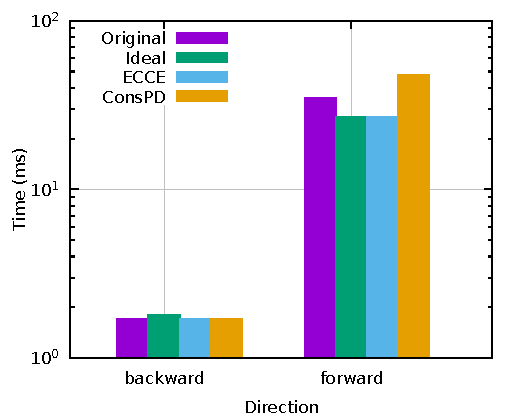
\includegraphics[width=\textwidth]{../data/doubleAppendo/da700log.pdf}
  \end{subfigure}
    \caption{Evaluation results for doubleAppendo}
    \label{tbl:doubleApp}
\end{figure}

\subsection{Maximal Element and Length of a List}

\begin{figure*}[!t]
  \centering
  \begin{minipage}{0.85\textwidth}
\begin{lstlisting}[label={cpd:maxandlength}, caption={Maximum element and length of the list}, captionpos=b, frame=tb]
  let maxLength$^o$ xs m l = max$^o$ xs m /\ length$^o$ xs l
  let rec length$^o$ xs l = fresh (h t m) ( conde [
      (xs === []    /\ l === zero);
      (xs === h % t /\ l === succ m /\  length$^o$ t m)])

  let max$^o$ xs m = max$_1^o$ xs zero m
  let rec max$_1^o$ xs n m = fresh (h t) ( conde [
      (xs === []     /\  m === n);
      (xs === h % t) /\ (conde [
        (le$^o$ h n ^true /\  max$_1^o$ t n m);
        (gt$^o$ h n ^true /\  max$_1^o$ t h m)])])

  let rec le$^o$ x y b = fresh (x$_1$ y$_1$) ( conde [
      (x === zero    /\ b === ^true);
      (x === succ x$_1$ /\  y === zero    /\ b === ^false);
      (x === succ x$_1$ /\  y === succ y$_1$ /\  le$^o$ x$_1$ y$_1$ b)])
  let rec gt$^o$ x y b = fresh (x$_1$ y$_1$) ( conde [
      (x === zero    /\ b === ^false);
      (x === succ x$_1$ /\  y === zero    /\ b === ^true);
      (x === succ x$_1$ /\  y === succ y$_1$ /\  gt$^o$ x$_1$ y$_1$ b)])
  \end{lstlisting}
\end{minipage}
  \begin{minipage}{0.8\textwidth}
\begin{lstlisting}[label={ideal:maxandlength}, caption={Ideal implementation of maxlengtho}, captionpos=b, frame=tb]
  let maxLength$^o$ xs m l = maxLength$_1^o$ xs m zero l
  let rec maxLength$_1^o$ xs m n l = fresh (h t l$_1$) ( conde [
      ( xs === []     /\  m === n        /\ l === zero);
      ((xs === h % t) /\ (l === succ l$_1$) /\  (conde [
         (le$^o$ h n ^true /\  maxLength$_1^o$ t m n l);
         (gt$^o$ h n ^true /\  maxLength$_1^o$ t m h l)]))])
  \end{lstlisting}
\end{minipage}
\end{figure*}

\begin{figure}[!h]
  \begin{subfigure}[c]{0.4\textwidth}
    \centering
    \begin{tabular}{c||c}
      & [1..100] \\ \hline\hline
      Original         & 48.5ms  \\ \hline
      Ideal            & 32.2ms  \\ \hline
      Ideal removed    & 19.6ms  \\ \hline
      \ecce            & 23.7ms  \\ \hline
      ConsPD          & 35.7ms
    \end{tabular}
  \end{subfigure}
  \hfill
  \begin{subfigure}[c]{0.45\textwidth}
    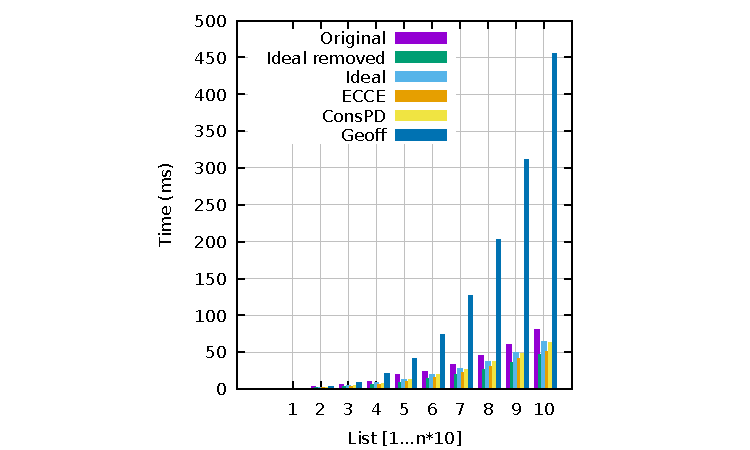
\includegraphics[width=\textwidth]{../data/maxLengtho/max.pdf}
  \end{subfigure}
  \caption{Execution time of maxlengtho}
  \label{tbl:maxlen}
\end{figure}

The relation \lstinline{maxLenght$^o$} computes the maximal element of the input list and its length (see Listing~\ref{cpd:maxandlength}) by conjunction of two relation calls.
The list \lstinline{xs} is traversed twice: first to compute the maximum in the relation \lstinline{max$^o$} and then to compute the length in the relation \lstinline{length$^o$}.
The input list contain Peano numbers which are compared by relations less-or-equal (\lstinline{le$^o$}) and greater-than (\lstinline{gt$^o$}).
Note that the comparison relations have three arguments with the last one representing the result of comparison.

The ideal implementation provided in the CPD literature~\cite{de1999conjunctive} is shown on Listing~\ref{ideal:maxandlength}.
This implementation traverses the input list \lstinline{xs} only once and can be generated by tupling.
Note, the disjunct which unifies the third argument with \lstinline{^false}\footnote{An arrow lifts ordinary values to the logic domain} in the implementation of both \lstinline{le$^o$} and \lstinline{gt$^o$} can never contribute into the result of \lstinline{maxLength$^o$} execution.
Such disjuncts are removed by both \ecce and conservative partial deduction, thus we consider two ideal implementions: one with the original comparison relations (\emph{Ideal}) and another in which these disjuncts are deleted (\emph{Ideal removed}).

We measured the execution time of \lstinline{maxLength$^o$ lst m l}, where \lstinline{lst} is a list of Peano numbers from $1$ to $100$.
The results are presented in Fig.~\ref{tbl:maxlen}.

Both \ecce and ConsPD improve the performance of \lstinline{maxLength$^o$} as compared to the original program.
Removing the disjuncts with the result unified with \lstinline{^false} in the comparison relations improves the ideal program by about 40\%.
ConsPD removes disjuncts which never succeed, but does not perform tupling, thus its result is not as performant as the ideal program.


\subsection{Evaluator of Logic Formulas}

The relation \lstinline{eval$^o$} describes an evaluation of a propositional formula under given variable assignments.
The relation has three arguments. The first argument is a list of boolean values which plays a role of variable assignments.
The $i$-th value of the substitution is the value of the $i$-th variable.
The second argument is a formula with the following abstract syntax.
A formula is either a \emph{variable} represented with a Peano number, a \emph{negation} of a formula, a \emph{conjunction} of two formulas or a \emph{disjunction} of two formulas.
The third argument is the value of the formula under the given assignment.

We specialize the \lstinline{eval$^o$} relation to synthesize formulas which evaluate to \lstinline{^true}.
To do so, we run the specializer for the goal with the last argument fixed to \lstinline{^true}, while the first two arguments remain free variables.
Depending on the way the \lstinline{eval$^o$} is implemented, different specializers generate significantly different residual programs.

\subsubsection{The Order of Relation Calls.}

One possible implementation of the evaluator is presented in Listing~\ref{eval:last}.
Here the relation \lstinline{elem$^o$ subst v res} unifies \lstinline{res} with the value of the variable \lstinline{v} in the list \lstinline{subst}.
The relations \lstinline{and$^o$}, \lstinline{or$^o$}, and \lstinline{not$^o$} encode corresponding boolean connectives.

\begin{figure*}[!t]
  \centering
  \begin{minipage}{0.95\textwidth}
    \begin{lstlisting}[label={eval:last}, caption={Evaluator of formulas with boolean operation last}, captionpos=b, frame=tb]
  let rec eval$^o$ subst fm res = conde [fresh (x y z v w) (
      (fm === var v    /\ elem$^o$ subst v res);
      (fm === conj x y /\ eval$^o$ st x v /\  eval$^o$ st y w /\  and$^o$ v w res);
      (fm === disj x y /\ eval$^o$ st x v /\  eval$^o$ st y w /\  or$^o$   v w res);
      (fm === neg x    /\ eval$^o$ st x v /\  not$^o$ v res))]
    \end{lstlisting}
  \end{minipage}
  \begin{minipage}{0.95\textwidth}
    \begin{lstlisting}[label={eval:fst}, caption={Evaluator of formulas with boolean operation second}, captionpos=b, frame=tb]
  let rec eval$^o$ subst fm res = conde [fresh (x y z v w) (
      (fm === var v    /\ elem$^o$ subst v res);
      (fm === conj x y /\ and$^o$ v w res /\  eval$^o$ st x v /\  eval$^o$ st y w);
      (fm === disj x y /\ or$^o$   v w res /\ eval$^o$ st x v /\  eval$^o$ st y w);
      (fm === neg x    /\ not$^o$ v res   /\ eval$^o$ st x v))]
    \end{lstlisting}
  \end{minipage}
\end{figure*}

Note, the calls to boolean relations \lstinline{and$^o$}, \lstinline{or$^o$}, and \lstinline{not$^o$} are placed last within each conjunction.
This poses a challenge for the CPD-based specializers such as \ecce.
Conjunctive partial deduction unfolds relation calls from left to right, so when specializing this relation for running backwards (i.e. considering the goal \lstinline{eval$^o$ subst fm ^true}), it fails to propagate the direction data onto recursive calls of \lstinline{eval$^o$}.
Knowing that \lstinline{res} is \lstinline{^true}, we can conclude that in the call \lstinline{and$^o$ v w res} variables \lstinline{v} and \lstinline{w} have to be \lstinline{^true} as well.
There are three possible options for these variables in the call \lstinline{or$^o$ v w res} and one for the call \lstinline{not$^o$}.
These variables are used in recursive calls of \lstinline{eval$^o$} and thus restrict the result of driving.
CPD fails to recognize this, and thus unfolds recursive calls of \lstinline{eval$^o$} applied to fresh variables.
It leads to over-unfolding, large residual programs and poor performance.

The conservative partial deduction first unfolds those calls which are selected according to the heuristics.
Since exploring the implementations of boolean connectives makes more sense, they are unfolded before recursive calls of \lstinline{eval$^o$}.
The way conservative partial deduction treats this program is the same as it treats the other implementation in which boolean connectives
are moved to the left, as shown in Listing~\ref{eval:fst}.
This program is easier for \ecce to specialize which demonstrates how unequal the behaviour of CPD for similar programs is.

\subsubsection{Unfolding of Complex Relations.}

Depending on the way a relation is implemented, it may take a different number of driving steps to reach the point when any useful information is derived through its unfolding.
Partial deduction tries to unfold every relation call unless it is unsafe, but not all relation calls serve to restrict the search space and thus should be unfolded.
In the implementation of \lstinline{eval$^o$} boolean connectives can effectively restrict variables within the conjunctions and should be unfolded until they do.
But depending on the way they are implemented, the different number of driving steps should be performed for that.
The simplest way to implement these relations is by mimicking a truth tables as demonstrated by the implementation of \lstinline{not$^o$} in Listing~\ref{not:table}.
It is enough to unfold such relation calls once to derive useful information about variables.

\begin{figure*}[!t]
  \centering
  \begin{minipage}{0.7\textwidth}
    \begin{lstlisting}[label={not:table}, caption={Implementation of boolean \lstinline{not} as a table}, captionpos=b, frame=tb]
  let not$^o$ x y = conde [
     (x === ^true /\ y === ^false;
      x === ^false /\ y === ^true)]
    \end{lstlisting}
  \end{minipage}
  \begin{minipage}{0.9\textwidth}
    \begin{lstlisting}[label={not:nando}, caption={Implementation of boolean operation via \lstinline{nand}}, captionpos=b, frame=tb]
  let not$^o$   x y = nand$^o$ x x y
  let or$^o$   x y z = nand$^o$ x x xx /\  nand$^o$ y y yy /\ nand$^o$ xx yy z
  let and$^o$ x y z = nand$^o$ x y xy /\   nand$^o$ xy xy z
  let nand$^o$ a b c = conde [
    ( a === ^false /\ b === ^false /\ c === ^true );
    ( a === ^false /\ b === ^true  /\ c === ^true );
    ( a === ^true  /\ b === ^false /\ c === ^true );
    ( a === ^true  /\ b === ^true  /\ c === ^false)]
    \end{lstlisting}
  \end{minipage}
\end{figure*}

The other way to implement boolean connectives is to express them using a single basic boolean relation such as \lstinline{nand$^o$} which is, in turn, has a table-based
implementation (see Listing~\ref{not:nando}). It will take several sequential unfoldings to derive that variables \lstinline{v} and \lstinline{w} should
be \lstinline{^true} when considering a call \lstinline{and$^o$ v w ^true} implemented via a basic relation.
Conservative partial deduction drives the selected call until it derives useful substitutions for the variables involved while CPD with deterministic unfolding may fail to do so.

\subsubsection{Evaluation Results.}
In our study we considered four implementations of \lstinline{eval$^o$}:
\begin{itemize}
  \item \emph{FirstPlain} in which the implementations of boolean connectives are \textbf{table-based} and are placed \textbf{before} recursive calls to \lstinline{eval$^o$}
  \item \emph{LastPlain} in which the implementations of boolean connectives are \textbf{table-based} and are placed \textbf{after} recursive calls to \lstinline{eval$^o$}
  \item \emph{FirstNando} in which boolean connectives are implemented via \lstinline{nand$^o$} and are placed \textbf{before} recursive calls to \lstinline{eval$^o$}
  \item \emph{LastNando} in which boolean connectives are implemented via \lstinline{nand$^o$} andare placed \textbf{after} recursive calls to \lstinline{eval$^o$}

\end{itemize}

These four implementations are very different from \ecce standpoint.
We measured the time necessary to generate $1000$ formulas over two variables which evaluate to \lstinline{^true} (averaged over 10 runs).
The results are presented in Fig.~\ref{tbl:eval}.

\begin{figure}[!t]
  \centering
  \begin{subfigure}[c]{0.35\textwidth}
    \centering
    %% \begin{tabular}{c||c|c|c|c}
    %%   & FirstPlain & FirstNando & LastPlain & LastNando \\ \hline\hline
    %%   Original         & 14.8ms     & 14.5ms     & 7.4ms     & 10.1ms    \\ \hline
    %%   \ecce            & 16.0ms     & 22.3ms     & 14.0ms    & 14.9ms    \\ \hline
    %%   ConsPD          & 9.1ms      & 9.7ms      & 9.1ms     & 9.9ms     \\
    %% \end{tabular}
    \begin{tabular}{e{1cm}||c|c|c}
      & Original & \ecce  & ConsPD \\ \hline\hline
      FirstPlain & 14.8ms & 16.0ms & 9.1ms \\ \hline
      FirstNando & 14.5ms & 22.3ms & 9.7ms \\ \hline
      LastPlain  & 7.4ms  & 14.0ms & 9.1ms \\ \hline
      LastNando  & 10.1ms & 14.9ms & 9.9ms
    \end{tabular}
  \end{subfigure}
  \hfill
  \begin{subfigure}[c]{0.6\textwidth}
    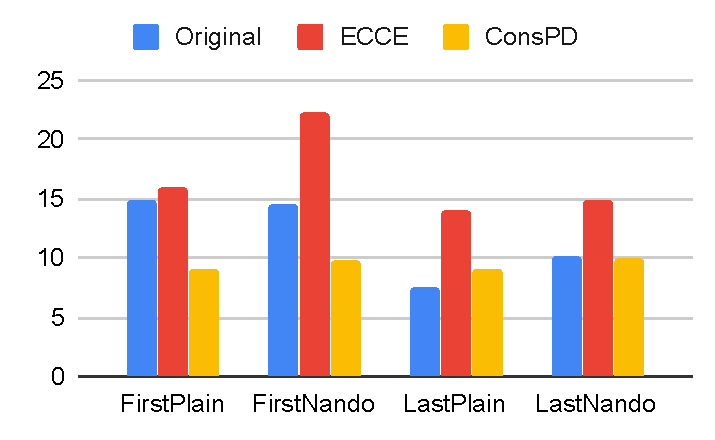
\includegraphics[width=\textwidth]{../data/propEval/prop.pdf}
  \end{subfigure}
  \caption{Execution time of evalo}
  \label{tbl:eval}
\end{figure}

ConsPD generates programs with comparable performance for all four implementations, while the quality of \ecce specialization differs significantly.
\ecce worsens performance for every implementation as compared to the original program.
ConsPD worsens performance of only the fastest implementation \emph{LastPlain}, while improving it for others.


\subsection{Typechecker-Term Generator}

This relation implements a typechecker for a tiny expression language.
Being executed in the backward direction it serves as a generator of terms of the given type.
The abstract syntax of the language is presented below.
The variables are represented with de Bruijn indices, thus let-binding does not specify which variable is being bound.

\[\begin{array}{lllll}
  type \ term = &\ BConst \ of \ Bool &| \ IConst \ of \ Int &| \ Var \ of \ Int & \\
  & | \ term + term &| \ term * term &| \ term = term &| \ term < term \\
  &| \ \underline{let} \ term \ \underline{in} \ term
  &\multicolumn{2}{l}{| \ \underline{if} \ term \ \underline{then} \ term \ \underline{else} \ term} &
\end{array}\]

The typing rules are straightforward and are presented below.
Boolean and integer constants have the corresponding types regardless of the environment.
Only terms of type integer can be summed up, multiplied or compared by less-than operator.
Any terms of the same type can be checked for equality.
Addition and multiplication of two terms of suitable types have integer type, while comparisons have boolean type.
If-then-else expression typechecks only if its condition is of type boolean, while both then- and else-branches have the same type.
An environment $\Gamma$ is an ordered list, in which the $i$-th element is the type of the variable with the $i$-th de Bruijn index.
To typecheck a let-binding, first, the term being bound is typechecked and is added in the beginning of the environment $\Gamma$, and then the body is typechecked in the context of the new environment.
Typechecking a variable with the index $i$ boils down to getting an $i$-th element of the list.

\begin{figure*}[!h]
  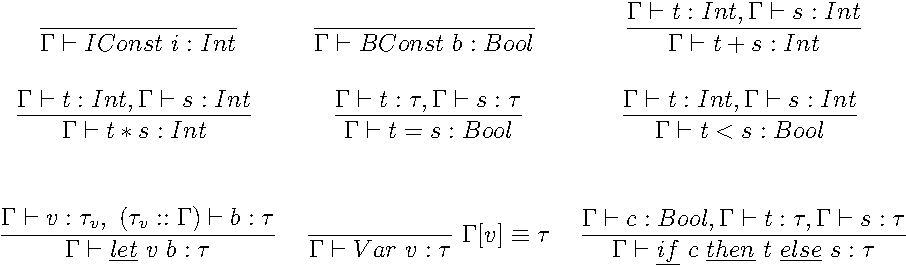
\includegraphics[width=\textwidth]{typechecker-crop.pdf}
\end{figure*}

We compared two implementations of these typing rules.
The first one is obtained by unnesting of the functional program as described in~\cite{lozov2019relational} (\emph{Generated}).
The second program is hand-written in \oc (\emph{Hand-written}).
Each implementation has been specialized with ConsPD and \ecce.
We measured the time needed to generate 1000 closed terms of type integer (averaged over 10 iterations; see Table~\ref{tbl:eval}).

\begin{table}
  \centering
  \begin{tabular}{c||c||c}
              & Hand-written & Generated \\ \hline\hline
  Original    & 916.9ms      & 11458.6ms \\ \hline
  ConsPD      & 335.9ms      & 289.8ms   \\ \hline
  \ecce       & 218.6ms      & 382.0ms   \\
  \end{tabular}
  \caption{Execution  time of generating 1000 closed terms of type Integer}
  \label{tbl:eval}
\end{table}

Note that the generated program is far slower than hand-written.
The principal difference between these two implementations is that the generated program contains a certain redundancy.
For example, typechecking of the sum of two terms in the hand-written implementation is implemented by a single conjunction (see Listing~\ref{type:hand}) while the generated program is far more complicated and also uses a special relation \lstinline{typeEq$^o$} to compare types (see Listing~\ref{type:gen}).


\begin{figure*}[!t]
  \centering
  \begin{minipage}{0.95\textwidth}
    \begin{lstlisting}[label={type:hand}, caption={A fragment of hand-written typechecker}, captionpos=b, frame=tb]
  let rec typecheck$^o$ gamma term res = conde [
    ...
    fresh (x y) ((term === x + y /\
       typecheck$^o$ gamma x ^(Some Integer) /\
       typecheck$^o$ gamma y ^(Some Integer) /\
       res === ^(Some Integer)));
    ...]
    \end{lstlisting}
  \end{minipage}

  \begin{minipage}{0.95\textwidth}
    \begin{lstlisting}[label={type:gen}, caption={A fragment of generated typechecker}, captionpos=b, frame=tb]
let rec typecheck$^o$ gamma term res = conde [
  ...
  fresh (x y t1 t2) ((term === x + y /\
    conde [
      typecheck$^o$ gamma x ^None       /\ res === ^None;
      typecheck$^o$ gamma x ^(Some t1) /\
        typecheck$^o$ gamma y ^None     /\ res === ^None;
      typecheck$^o$ gamma x ^(Some t1) /\  typecheck$^o$ gamma y ^(Some t2) /\
        typeEq$^o$ t1 Integer ^true    /\ typeEq$^o$ t2 Integer ^true /\
        res === ^(Some Integer);
    ])
  ...]
    \end{lstlisting}
  \end{minipage}
\end{figure*}

Most of the redundancy of the generated program is removed by specialization with respect to the known type of the term.
This is why both implementations have comparable speed after specialization.
\ecce shows bigger speedup for the hand-written than ConsPD and vice versa for the generated implementation.
We believe that this difference can be explained by too much unfolding.
\ecce performs a lot of excessive unfolding for the generated program and only barely changes the hand-written program.
At the same time ConsPD specializes both implementations to comparable programs performing average amount of unfolding.
This shows that the heuristics we presented gives more stable, although not the best, results.

\subsection{Unification and Path Search}

Besides evaluator of logic formulas we also run the specializers on the relation \lstinline{unify$^o$}, which searches for a unifier of two terms, and a relation \lstinline{isPath$^o$},
used to search for paths in the graph.
Both relations were generated from functional programs by unnesting.
These two relations are described in paper~\cite{lozov2019relational} so we will not go into too many details here.

The \lstinline{unify$^o$} relation was executed to find a unifier of three pairs of terms (see table~\ref{tbl:unify}) which vary in their complexity.
The original program failed to terminate on two last unification problems in under 30s, while both ConsPD and \ecce generate programs which are able to find the unifiers.

\begin{table}
  \centering
  \begin{tabular}{c||c|c|c||c}
    & \multicolumn{3}{c||}{unify$^o$} & \\
    \multirow{2}{*}{Terms} & f(X, a) & f(a \% b \% nil, c \% d \% nil, L) & f(X, X, g(Z, t)) & \multirow{2}{*}{isPath$^o$}  \\
    \cline{2-4} &
    f(a, X) & f(X \% XS, YS, X \% ZS) & f(g(p, L), Y, Y)  \\
    \hline\hline
  Original          & 0.23ms &  ---   &  ---    & 24.9ms \\ \hline
  ConsPD            & 0.07ms & 16.5ms & 397.6ms & 1.6ms  \\ \hline
  \ecce             & 0.12ms & 18.8ms & 352.0ms & 1.1ms  \\ \hline
  \end{tabular}

  \caption{Evaluation results of unification and path search}
  \label{tbl:unify}
\end{table}

The relation \lstinline{isPath$^o$} was executed to search for 3 paths of length 7 in the graph with 20 vertices and 30 edges (see Table~\ref{tbl:unify}).
Both specializers significantly improve the performance as compared to the original program, although ConsPD is about 30\% worse than \ecce.
